\documentclass[11pt,a4paper,oneside]{article}
\usepackage[utf8]{inputenc}
\usepackage[T1]{fontenc}
\usepackage[french]{babel}
\usepackage{lmodern}
\usepackage{microtype}
\usepackage[a4paper,margin=2.25cm,headheight=15pt,footskip=28pt]{geometry}
\usepackage{amsmath,amssymb,amsthm,mathtools}
\usepackage{booktabs,tabularx,array}
\usepackage[dvipsnames]{xcolor}
\usepackage{tikz}
\usepackage{graphicx}
\usetikzlibrary{arrows.meta,calc,intersections,angles,quotes,patterns,positioning,decorations.pathreplacing}
\usepackage{fancyhdr}
\usepackage{hyperref}
\usepackage{enumitem}

\definecolor{Forest}{HTML}{1D5B4A}
\definecolor{Ink}{HTML}{16211D}
\definecolor{Mist}{HTML}{EAF0EC}
\definecolor{Muted}{HTML}{5B6862}
\hypersetup{colorlinks=true,linkcolor=Forest,urlcolor=Forest,citecolor=Forest,pdftitle={Curiosité mathématique},pdfauthor={Germain-Junior TWAMBA}}
\urlstyle{same}
\setlength{\parskip}{0.45em}
\setlength{\parindent}{0pt}
\setlist[enumerate]{leftmargin=2em,itemsep=0.25em,topsep=0.3em}
\setlist[itemize]{leftmargin=1.5em,itemsep=0.2em,topsep=0.3em}
\pagestyle{fancy}
\fancyhf{}
\fancyhead[L]{\small\textcolor{Muted}{Curiosités mathématiques}}
\fancyhead[R]{\small\textcolor{Muted}{Club des Divergents}}
\fancyfoot[C]{\small\textcolor{Muted}{\thepage}}
\renewcommand{\headrulewidth}{0.35pt}
\renewcommand{\footrulewidth}{0pt}
\newtheorem{theoreme}{Théorème}[section]
\newtheorem{proposition}[theoreme]{Proposition}
\newtheorem{lemme}[theoreme]{Lemme}
\theoremstyle{definition}
\newtheorem{definition}[theoreme]{Définition}
\newtheorem{exemple}[theoreme]{Exemple}
\newcommand{\titreDossier}[3]{%
  \begin{titlepage}\centering\vspace*{1.3cm}
  {\large\scshape\textcolor{Forest}{Club des Divergents \textbullet{} Goma, RDC}}\\[1.5cm]
  {\color{Forest}\rule{0.82\textwidth}{1.2pt}}\\[0.8cm]
  {\Huge\bfseries\sffamily\color{Ink}#1\par}\vspace{0.7cm}
  {\Large\color{Forest}#2\par}\vspace{1.2cm}
  {\large\color{Muted}Dossier de curiosité mathématique\par}
  \vfill
  \begin{minipage}{0.78\textwidth}\centering\large #3\end{minipage}
  \vfill
  {\color{Forest}\rule{0.82\textwidth}{1.2pt}}\\[0.45cm]
  {\large Germain-Junior TWAMBA\par}
  {\normalsize 13 novembre 2026\par}
  \end{titlepage}}
\newcommand{\sourceweb}[2]{\item \textbf{#1.} \url{#2}}
\newcommand{\idee}[1]{\begin{quote}\small\colorbox{Mist}{\parbox{0.94\linewidth}{\textbf{Idée à retenir.} #1}}\end{quote}}
\newcommand{\demonstration}{\par\smallskip\noindent\textbf{Démonstration.}\ }
\newcommand{\finpreuve}{\hfill$\square$\par}

\begin{document}
\titreDossier{Les matrices de Gram}{Produits scalaires, dépendance linéaire et volumes}{
Une matrice de Gram condense toutes les longueurs et tous les angles d'une famille de vecteurs. Sa positivité, son rang et son déterminant révèlent la géométrie de la famille, même lorsque les coordonnées ambiantes ne sont pas connues.}

\section*{Une géométrie rangée dans une matrice}
Connaître seulement la longueur de plusieurs vecteurs ne suffit pas à connaître leur disposition. Il faut aussi connaître leurs produits scalaires, qui mesurent leur alignement relatif. À partir des produits scalaires, on construit une matrice symétrique appelée matrice de Gram. Elle contient exactement l'information nécessaire pour calculer la longueur de toute combinaison linéaire de ces vecteurs.

Soient $v_1,\ldots,v_m$ des vecteurs d'un espace euclidien réel. Leur matrice de Gram est
\[
 G=(\langle v_i,v_j\rangle)_{1\leq i,j\leq m}.
\]
La diagonale contient les carrés des normes $\|v_i\|^2$. Les coefficients hors diagonale contiennent les produits scalaires, donc renseignent sur les angles.

Le nom rappelle le mathématicien danois Jørgen Pedersen Gram (1850-1916). Cette photographie d'archive est un repère historique ; les propriétés étudiées dans ce dossier découlent des produits scalaires et sont démontrées indépendamment du portrait.
\begin{figure}[htbp]
\centering
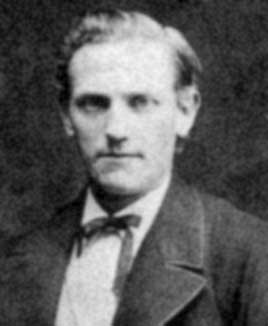
\includegraphics[height=3.5cm]{images/jorgen-gram.jpg}
\caption{Portrait d'archive de Jørgen Pedersen Gram (1850-1916), domaine public. La source d'origine et le photographe ne sont pas précisés dans la notice. Voir la \href{https://commons.wikimedia.org/wiki/File:Jorgen_Gram.jpg}{notice Wikimedia Commons}.}
\end{figure}

\begin{center}
\begin{tikzpicture}[scale=1.05,>=Latex]
  \coordinate (O) at (0,0); \coordinate (A) at (3.2,0.35); \coordinate (B) at (1.2,2.0); \coordinate (C) at (4.4,2.35);
  \draw[->,thick,Forest] (O)--(A) node[midway,below] {$v_1$};
  \draw[->,thick,BrickRed] (O)--(B) node[midway,left] {$v_2$};
  \draw[gray,thick] (A)--(C)--(B);
  \draw[dashed] (O)--(C);
  \draw (0.65,0.07) arc[start angle=6,end angle=59,radius=0.65];
  \node at (0.95,0.55) {$\theta$};
  \node[align=center] at (2,-0.85) {$\begin{gathered}\text{Aire du parall\'elogramme}\\=\sqrt{\det G}\end{gathered}$};
\end{tikzpicture}
\end{center}
\textit{Pour deux vecteurs, le déterminant de Gram est le carré de l'aire du parallélogramme qu'ils engendrent.}

\section{Définition et premières propriétés}
\begin{definition}
Dans un espace vectoriel muni d'un produit scalaire, la matrice de Gram d'une famille ordonnée $v_1,\ldots,v_m$ est la matrice $G$ telle que $G_{ij}=\langle v_i,v_j\rangle$.
\end{definition}

Dans un espace réel, $G$ est symétrique car $\langle v_i,v_j\rangle=\langle v_j,v_i\rangle$. Dans un espace complexe, on choisit une convention du produit hermitien et la matrice est hermitienne, c'est-à-dire $G^*=G$. Dans les deux cas, la structure fondamentale est la non-négativité de la forme quadratique associée.

\begin{proposition}
Pour tout vecteur de coefficients $c=(c_1,\ldots,c_m)^T$, on a
\[
 c^T Gc=\left\|\sum_{i=1}^m c_i v_i\right\|^2\geq0.
\]
Ainsi $G$ est positive semi-définie.
\end{proposition}

\demonstration Développons le carré de la norme à l'aide de la bilinéarité du produit scalaire :
\[
 \left\langle\sum_i c_iv_i,\sum_j c_jv_j\right\rangle
 =\sum_{i,j}c_ic_j\langle v_i,v_j\rangle=c^TGc.
\]
Une norme au carré ne peut être négative.\finpreuve

\section{Positivité stricte, rang et dépendance}
\begin{theoreme}
La matrice de Gram $G$ est définie positive si et seulement si les vecteurs $v_1,\ldots,v_m$ sont linéairement indépendants.
\end{theoreme}

\demonstration Si les vecteurs sont indépendants et $c\ne0$, la combinaison $\sum_i c_iv_i$ n'est pas nulle. Sa norme au carré est strictement positive, donc $c^TGc>0$. Réciproquement, si les vecteurs sont dépendants, il existe un $c\ne0$ tel que $\sum_i c_iv_i=0$. Alors $c^TGc=0$, donc la forme quadratique n'est pas définie positive.\finpreuve

La preuve donne même une équivalence de noyaux. Soit $V$ la matrice dont les colonnes sont les coordonnées des $v_i$. Alors $G=V^TV$, et
\[
 c^TGc=\|Vc\|^2.
\]
Par conséquent, $Gc=0$ si et seulement si $Vc=0$ : le noyau de $G$ décrit exactement les relations linéaires entre les vecteurs. Ainsi
\[
 \operatorname{rang}(G)=\dim\operatorname{Vect}(v_1,\ldots,v_m).
\]

Pour une famille de $m$ vecteurs, $\det G>0$ exactement lorsque les vecteurs sont indépendants ; si elle est dépendante, $\det G=0$. Toute matrice de Gram est symétrique et semi-définie positive. Réciproquement, toute matrice symétrique semi-définie positive $S$ est une matrice de Gram. Le théorème spectral donne $S=Q\Lambda Q^T$ avec $Q$ orthogonale et $\Lambda$ diagonale à coefficients $\geq0$ ; la matrice $V=\Lambda^{1/2}Q^T$ vérifie $V^TV=S$, et ses colonnes sont des vecteurs dont les produits scalaires sont les coefficients de $S$. Cette remarque relie le problème de représentation géométrique à l'algèbre linéaire.

\subsection{Cauchy-Schwarz depuis une matrice \texorpdfstring{$2\times2$}{2x2}}
Pour deux vecteurs, posons $a=\|u\|^2$, $b=\langle u,v\rangle$, $c=\|v\|^2$. La positivité de
\[
 G=\begin{pmatrix}a&b\\b&c\end{pmatrix}
\]
impose $\det G=ac-b^2\geq0$. Donc
\[
 |\langle u,v\rangle|\leq\|u\|\,\|v\|.
\]
L'égalité a lieu exactement lorsque $\det G=0$, c'est-à-dire lorsque $u$ et $v$ sont liés. L'inégalité de Cauchy-Schwarz est donc une conséquence directe de la positivité du Gram.

\section{Le déterminant de Gram mesure un volume}
\begin{theoreme}[Formule du volume]
Si $v_1,\ldots,v_m$ sont des vecteurs d'un espace euclidien et si $G$ est leur matrice de Gram, le volume $m$-dimensionnel du parallélotope qu'ils engendrent est
\[
 \boxed{\operatorname{Vol}_m(v_1,\ldots,v_m)=\sqrt{\det G}}.
\]
\end{theoreme}

\demonstration Supposons d'abord les vecteurs indépendants et plaçons leurs coordonnées, dans une base orthonormée de leur sous-espace (de dimension $m$), dans les colonnes d'une matrice carrée $V$. Le volume du parallélotope est $|\det V|$. Or $G=V^TV$, donc
\[
 \det G=\det(V^T)\det(V)=(\det V)^2.
\]
La racine carrée positive donne le volume. Si les vecteurs sont dépendants, les deux membres sont nuls : le parallélotope est aplati et $G$ est singulière.\finpreuve

Dans un espace ambiant de dimension supérieure à $m$, on peut choisir une base orthonormée du sous-espace engendré ; la preuve s'y applique sans changer les produits scalaires. La formule ne dépend donc pas de la dimension dans laquelle la figure est dessinée.

\subsection{Deux vecteurs et l'angle}
Si $\|u\|=a$, $\|v\|=b$ et l'angle entre eux vaut $\theta$, alors
\[
 G=\begin{pmatrix}a^2&ab\cos\theta\\ab\cos\theta&b^2\end{pmatrix},\qquad
 \det G=a^2b^2(1-\cos^2\theta)=a^2b^2\sin^2\theta.
\]
Ainsi l'aire vaut $ab|\sin\theta|$. Deux vecteurs presque parallèles donnent un déterminant petit ; s'ils sont exactement parallèles, l'aire et le déterminant sont nuls.

\section{Exemples calculés}
\subsection{Un parallélogramme}
Prenons dans $\mathbb R^2$ les vecteurs $u=(2,0)$ et $v=(1,3)$. Leurs produits scalaires sont
\[
 \langle u,u\rangle=4,\qquad \langle u,v\rangle=2,\qquad \langle v,v\rangle=10,
\]
donc
\[
 G=\begin{pmatrix}4&2\\2&10\end{pmatrix},\qquad \det G=40-4=36.
\]
L'aire du parallélogramme est $\sqrt{36}=6$. Le calcul direct confirme : le déterminant de la matrice des colonnes $(u,v)$ vaut $\det\begin{pmatrix}2&1\\0&3\end{pmatrix}=6$.

\subsection{Trois vecteurs dans l'espace}
Considérons
\[
 u=(1,1,0),\qquad v=(0,1,1),\qquad w=(1,0,1).
\]
Chaque vecteur a une norme au carré égale à $2$, et chaque produit scalaire entre deux vecteurs distincts vaut $1$. La matrice de Gram est
\[
 G=\begin{pmatrix}2&1&1\\1&2&1\\1&1&2\end{pmatrix}.
\]
Un calcul direct donne $\det G=4$. Le volume du parallélépipède est donc $2$. La matrice n'est pas diagonale, ce qui signifie que les vecteurs ne sont pas orthogonaux ; pourtant son déterminant donne exactement le volume sans construire d'altitude.

\subsection{Une famille dépendante}
Reprenons $u=(1,1,0)$, $v=(0,1,1)$ et posons cette fois $w=u+v=(1,2,1)$. La famille $(u,v,w)$ est liée et
\[
 G=\begin{pmatrix}2&1&3\\1&2&3\\3&3&6\end{pmatrix},\qquad \det G=0.
\]
Le vecteur $c=(1,1,-1)^T$ décrit la relation $u+v-w=0$ et vérifie bien $Gc=0$. Le volume tridimensionnel est nul : les trois vecteurs restent dans le plan engendré par $u$ et $v$.

\section{Applications et connexions}
\subsection{Projection et moindres carrés}
Soit $V$ une matrice dont les colonnes forment une famille indépendante. Pour approcher un vecteur $b$ par $Vc$, on minimise $\|Vc-b\|^2$. Le gradient vaut $2V^T(Vc-b)$ ; en l'annulant, on obtient les équations normales
\[
 V^TVc=V^Tb,
\]
soit $Gc=V^Tb$. La matrice de Gram gouverne donc les projections orthogonales et les problèmes de moindres carrés. Si les colonnes sont presque dépendantes, $G$ est mal conditionnée : de petites perturbations des données peuvent entraîner de grands changements des coefficients $c$.

\subsection{Distance à partir des produits scalaires}
La distance entre deux vecteurs se récupère par
\[
 \|u-v\|^2=\langle u,u\rangle+\langle v,v\rangle-2\langle u,v\rangle.
\]
Un tableau de produits scalaires suffit ainsi à retrouver toutes les distances entre les vecteurs d'une famille. C'est pourquoi les Gram apparaissent en géométrie, en approximation numérique, en statistiques et dans les méthodes à noyau.

\subsection{Lien avec Gram-Schmidt et Cholesky}
Le procédé de Gram-Schmidt remplace une famille indépendante par une famille orthogonale ayant le même sous-espace engendré. Après ce changement triangulaire, le déterminant de Gram devient le produit des carrés des normes des vecteurs orthogonaux. Sur le plan algébrique, une matrice définie positive admet une factorisation de Cholesky $G=R^TR$ avec $R$ triangulaire supérieure. Les colonnes de $R$ fournissent une réalisation concrète, triangulaire, de la géométrie codée par $G$.

\section*{À retenir et exercices}
\begin{itemize}
 \item $G_{ij}=\langle v_i,v_j\rangle$ ; $G$ est symétrique ou hermitienne.
 \item $c^TGc=\|\sum c_iv_i\|^2$, donc $G$ est semi-définie positive.
 \item $\operatorname{rang}G$ est la dimension de l'espace engendré.
 \item $\sqrt{\det G}$ est le volume du parallélotope.
\end{itemize}
\begin{enumerate}
 \item Construisez la matrice de Gram de $(1,0,1)$ et $(1,1,0)$ dans $\mathbb R^3$ et calculez leur aire.
 \item Montrez que si deux vecteurs sont orthogonaux, leur matrice de Gram est diagonale.
 \item Expliquez pourquoi ajouter un vecteur déjà dans l'espace engendré ne peut pas augmenter le rang du Gram.
 \item Montrez que $\det G\leq\prod_i\|v_i\|^2$ (inégalité de Hadamard) et vérifiez-la sur l'exemple à trois vecteurs.
\end{enumerate}
\textbf{Réponses.}
\begin{enumerate}
 \item $G=\begin{pmatrix}2&1\\1&2\end{pmatrix}$, $\det G=3$, aire $\sqrt3$.
 \item Si $\langle u,v\rangle=0$, les coefficients hors diagonale sont nuls : $G=\operatorname{diag}(\|u\|^2,\|v\|^2)$.
 \item Le rang de $G$ est la dimension de l'espace engendré (section 2) ; un vecteur déjà dans cet espace ne la change pas.
 \item Le volume du parallélotope est au plus le produit des longueurs des côtés (Gram-Schmidt : chaque vecteur orthogonalisé est plus court que l'original), donc $\det G=\operatorname{Vol}^2\leq\prod\|v_i\|^2$. Pour l'exemple : $4\leq2\cdot2\cdot2=8$.
\end{enumerate}

\section*{Références}
\begin{enumerate}
 \sourceweb{University of Minnesota, \og Constructing positive definite or positive semidefinite matrices\fg{}, notes de cours}{https://www-users.cse.umn.edu/~rylai/docs1/teaching/math4242/S2021_M4242/Lecture20.pdf}
 \sourceweb{University of Colorado, \og Differential Geometry of Curves and Surfaces\fg{}, formule volume-déterminant de Gram}{https://math.colorado.edu/~casa/teaching/26fall/4230/lecture_notes/index.html}
 \sourceweb{Israel Halperin, \og On the Gram Matrix\fg{}, Canadian Mathematical Bulletin, 5(3), 1962}{https://doi.org/10.4153/CMB-1962-027-1}
\end{enumerate}
\end{document}
